\section{Halbordnungen}
Eine \emph{Halbordnung} (poset) ist eine homogene Relation $\preceq$ auf einer Menge $A$, die
\begin{itemize}
  \item \emph{reflexiv}: $\forall a\in A:\; a\preceq a$,
  \item \emph{transitiv}: $\forall a,b,c\in A:\; (a\preceq b \wedge b\preceq c)\Rightarrow a\preceq c$,
  \item \emph{antisymmetrisch}: $\forall a,b\in A:\; (a\preceq b \wedge b\preceq a)\Rightarrow a=b$.
\end{itemize}

\subsection{Typische Beispiele}
\begin{itemize}
  \item $(\mathcal{P}(A),\subseteq)$, die Mengeninklusion auf der Potenzmenge.
  \item Teilbarkeitsrelation auf $\mathbb{N}$.
  \item Die üblichen $\leq$-Relationen auf $\mathbb{N},\mathbb{Z},\mathbb{Q},\mathbb{R}$.
  \item Versionen in der Informatik, z.\,B. Commit-Historien in Git (Ursprungsrelation).
\end{itemize}

\subsection{Zyklenfreiheit}
In einer Halbordnung sind echte Zyklen ausgeschlossen: Aus
$a_1\preceq a_2\preceq\cdots\preceq a_n\preceq a_1$ folgt $a_1=\cdots=a_n$.
Dies folgt aus der Antisymmetrie und der Transitivität.

\subsection{Hasse-Diagramme}
Zur Visualisierung nutzt man Hasse-Diagramme:
\begin{itemize}
  \item Relative Höhe zeigt die Ordnungsrichtung.
  \item Kanten werden nur zwischen \emph{benachbarten} Elementen ohne Zwischenelement gezeichnet (Transitivitätskanten weglassen).
  \item Schleifen entfallen.
\end{itemize}

\textbf{Beispiele:} 
Hesse-Diagramm des Poset der Teilbarkeitsrelation auf 28 (\emph{Rechts}) und \((\mathcal{P}(\{a,b,c\}),\subseteq)\) (\emph{Links}):\\
\begin{tikzpicture}
    % Nodes
    \node (1) at (3,0) {1};
    \node (2) at (2,1) {2};
    \node (4) at (1,2) {4};
    \node (7) at (4,1) {7};
    \node (14) at (3,2) {14};
    \node (28) at (2,3) {28};
    
    % Edges
    \draw (1) -- (2);
    \draw (1) -- (7);
    \draw (2) -- (4);
    \draw (2) -- (14);
    \draw (7) -- (14);
    \draw (4) -- (28);
    \draw (14) -- (28);
\end{tikzpicture}
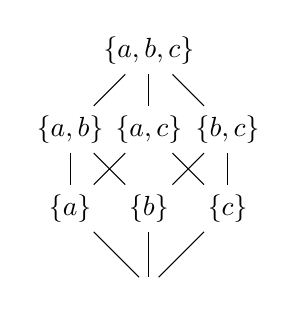
\begin{tikzpicture}
    % Nodes
    \node (empty) at (1,0) {$\varnothing$};
    \node (a) at (0,1) {$\{a\}$};
    \node (b) at (1,1) {$\{b\}$};
    \node (c) at (2,1) {$\{c\}$};
    \node (ab) at (0,2) {$\{a,b\}$};
    \node (ac) at (1,2) {$\{a,c\}$};
    \node (bc) at (2,2) {$\{b,c\}$};
    \node (abc) at (1,3) {$\{a,b,c\}$};

    % Edges
    \draw (empty) -- (a);
    \draw (empty) -- (b);
    \draw (empty) -- (c);
    \draw (a) -- (ab);
    \draw (a) -- (ac);
    \draw (b) -- (ab);
    \draw (b) -- (bc);
    \draw (c) -- (ac);
    \draw (c) -- (bc);
    \draw (ab) -- (abc);
    \draw (ac) -- (abc);
    \draw (bc) -- (abc);
\end{tikzpicture}


\subsection{Spezielle Elemente}
Sei $X\subseteq A$ in einer Halbordnung $(A,\preceq)$. Ein Element $x\in X$ heisst:
\begin{itemize}
  \item \textbf{minimales Element:} $\forall y\;(y\preceq x\Rightarrow y=x)$\\(Knoten zu \emph{denen} kein Pfeil zeigt)
  \item \textbf{kleinstes Element:} $\forall y\;(x\preceq y)$\\(Knoten von \emph{dem} ein Pfeil zu jedem anderen zeigt)
  \item \textbf{maximales Element:} $\forall y\;(x\preceq y\Rightarrow y=x)$\\(Knoten von \emph{denen} kein Pfeil ausgeht)
  \item \textbf{grösstes Element:} $\forall y\;(y\preceq x)$\\(Knoten zu \emph{dem} jeder Pfeil zeigt)
\end{itemize}

\subsubsection{Existenz in endlichen Mengen}
Ist $X\subseteq A$ nichtleer und endlich, so existiert mindestens ein minimales und mindestens ein maximales Element in $X$.

\subsubsection{Erweiterungen}
Eine Halbordnung $(A,\preceq_A)$ erweitert eine Halbordnung $(B,\preceq_B)$, wenn gilt:
  \[B \subseteq A,\]
  \[\forall a,b\in B (a\preceq_B b \Rightarrow a\preceq_A b).\]
Man sagt: $(A,\preceq_A)$ \emph{erweitert} $(B,\preceq_B)$.


\subsection{Lineare Ordnungen}

Eine \emph{lineare Ordnung} (auch \emph{totale Ordnung}) ist eine Halbordnung $(A,\preceq)$, in der alle Elemente vergleichbar sind:
\[
\forall a,b\in A(a\preceq b \lor b\preceq a).
\]
Das heisst, es gibt keine \emph{unvergleichbaren} Paare mehr.

\subsubsection{Satz von Marczewski--Szpilrajn}
Jede Halbordnung \((A,\preceq)\) lässt sich zu einer linearen Ordnung \((A,\unlhd)\) erweitern, die die ursprüngliche Ordnung bewahrt und \emph{alle} Elemente vergleichbar macht.

\subsection{Graphentheoretische Sicht}
\begin{itemize}
  \item Eine endliche Halbordnung kann als gerichteter azyklischer Graph (DAG) dargestellt werden.
  \item Eine \emph{Linearisierung} entspricht einer \emph{topologischen Sortierung} des DAGs.
\end{itemize}
